\clearpage %%% für Druck

\subsubsection{Wasserfallmodell(e)}
\label{sec:Kap-2.2.1.1}

\vspace{\baselineskip} %%% für Druck

\sttpLeserfuehrung{Bilder/Kapitel-2/Leserfuehrung/vorgehensmodelle_sequentiell_illustration.pdf}{Bilder/Kapitel-2/Leserfuehrung/vorgehensmodelle_wasserfall.pdf}

Die Überschrift deutet es schon an: Eigentlich ist es falsch von \textbf{dem} Wasserfallmodell zu sprechen, da es Wasserfallmodelle heute in vielen Varianten gibt. Dementsprechend unterschiedliche Abbildungen findet man in der Literatur.

\minisec{Historische Wasserfallmodelle} 

Das ursprüngliche Wasserfallmodell stellte Winston W. Royce 1970 vor \cite{roy70}. \mbox{Royce} orientierte sich für sein Modell an der Darstellung eines sequentiellen Prozessmodells aus den 1950er Jahren\footnote{Das sogenannte \textit{stagewise model}, ein Prozessmodell für die Systementwicklung des Semi-Automatic Ground Environment Systems (SAGE), das erste computergestützte Luftverteidigungssystem Nordamerikas (USA, Kanada). 1956 von Herbert D. Benington beschrieben \cite{ben56}, zusammenfassend zum Modell \cite[43\psq]{kne17}.}, verdichtete dessen ursprünglich neun Phasen zu sieben, ergänzte sogenannte Rückkopplungsmöglichkeiten (Rückkehr von einer Phase in die vorhergehende Phase) und führte die an einen Wasserfall erinnernde Darstellung ein. Abbildung~\ref{fig:wasserfallmodel_nach_royce} zeigt das Wasserfallmodell von Royce.  

\begin{figure}[h!]
    \centering
    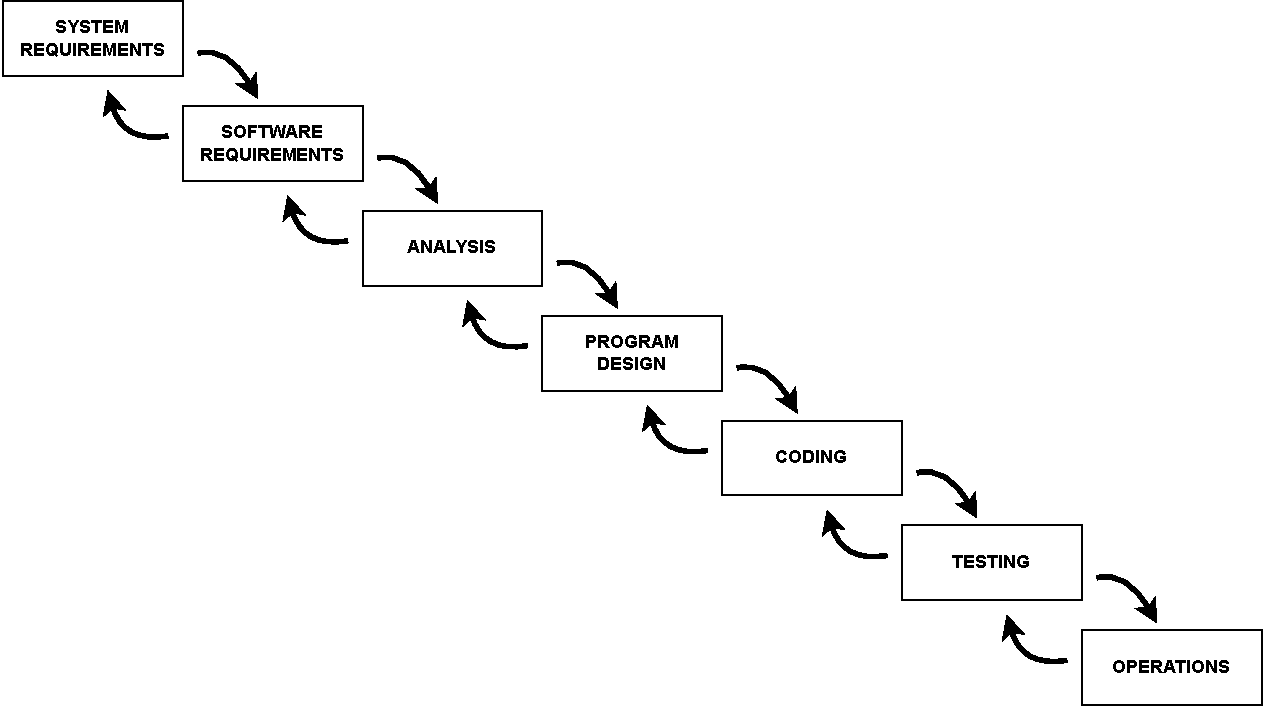
\includegraphics[width=1.0\textwidth]{Bilder/Kapitel-2/WasserfallmodellRoyce.pdf}
    \caption[Wasserfallmodell von Royce]{Wasserfallmodell von Royce, nach \cite[330]{roy70}}
    \label{fig:wasserfallmodel_nach_royce}
\end{figure}

\pagebreak %%% für Druck

In mancher Literatur findet sich die Unterscheidung zwischen einem Wasserfall\-modell \textbf{ohne} und einem Wasserfallmodell \textbf{mit} Rückkehrmöglichkeit in die vorhergehende Phase. Dies ist allerdings ein Irrtum, der darauf zurückzuführen ist, dass der Artikel von Royce zur Hinführung auf sein Modell auch wasserfallartige Abbildungen ohne Rückkehrmöglichkeiten enthält. Das von ihm vorgeschlagene Modell sieht die Rückkopplung zur jeweils vorhergehenden Phase aber explizit vor. Kaum in Erinnerung geblieben ist zudem, dass Royce eng verknüpft mit seinem Modell Maßnahmen zur Reduzierung von Entwicklungsrisiken vorschlägt, die man heute erst später entstandenen Vorgehensmodellen zuordnet. Dazu gehören eine kontinuier\-liche Einbeziehung der zukünftigen Nutzer (in Royce' Modell noch an festen Punkten im Projektablauf) und das Arbeiten mit Prototypen 
%\sttpgls{Prototyp}
(er verwendet den Begriff pilot model).

Vermehrt eingesetzt für die Softwareentwicklung werden Wasserfallmodelle seit den Veröffentlichungen von Barry W. Boehm  in den 1980er Jahren. Abbildung~\ref{fig:wasserfallmodel_nach_boehm} zeigt das Wasserfallmodell von Boehm.  

\begin{figure}[h!]
    \centering
    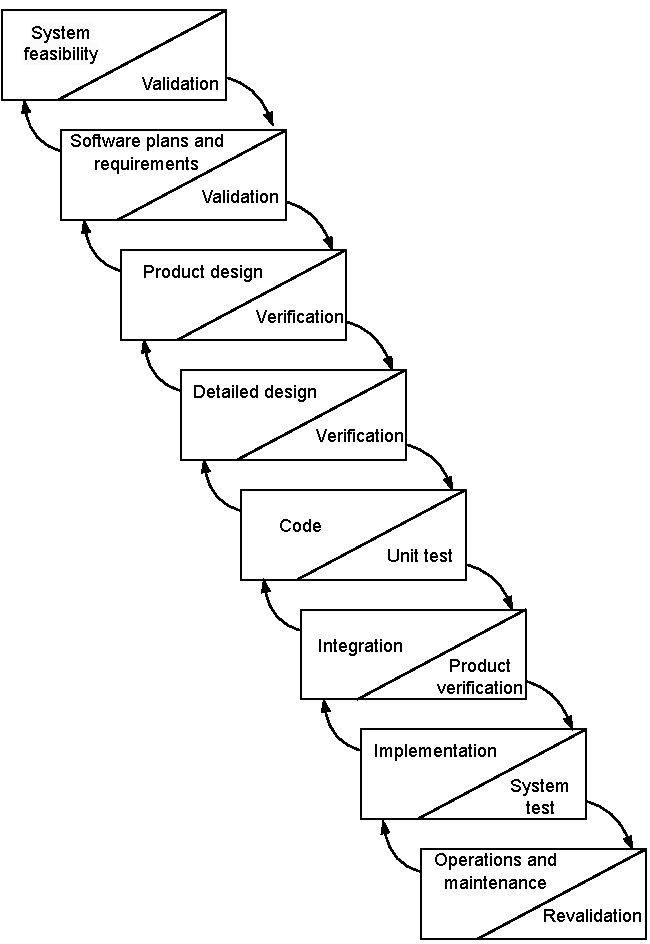
\includegraphics[scale=0.75]{Bilder/Kapitel-2/WasserfallmodellBoehm.pdf}
    \vspace{\baselineskip} %%% für Druck
    \caption[Wasserfallmodell von Boehm]{Wasserfallmodell von Boehm, nach \cite[36]{boe81}}
    \label{fig:wasserfallmodel_nach_boehm}
\end{figure}

\pagebreak %%% für Druck

Boehm erweiterte Anfang der 1980er Jahre das Modell von Royce, indem er den Zuschnitt der einzelnen Phasen veränderte, den Punkt der Softwarewartung (engl. maintenance) ergänzte und Qualitätssicherungsaspekte explizit ins Modell aufnahm. Boehm war zudem derjenige, der den Namen Wasserfallmodel populär machte.

\minisec{Heutige Wasserfallmodelle}

Heute findet man überwiegend fünf- und sechsphasige Wasserfallmodelle. Abbildung~\ref{fig:wasserfallmodel_fuenf_phasen} zeigt links ein beispielhaftes fünfphasiges Wasserfallmodell und rechts ein sechsphasiges. 

\begin{figure}[h!]
    \centering
		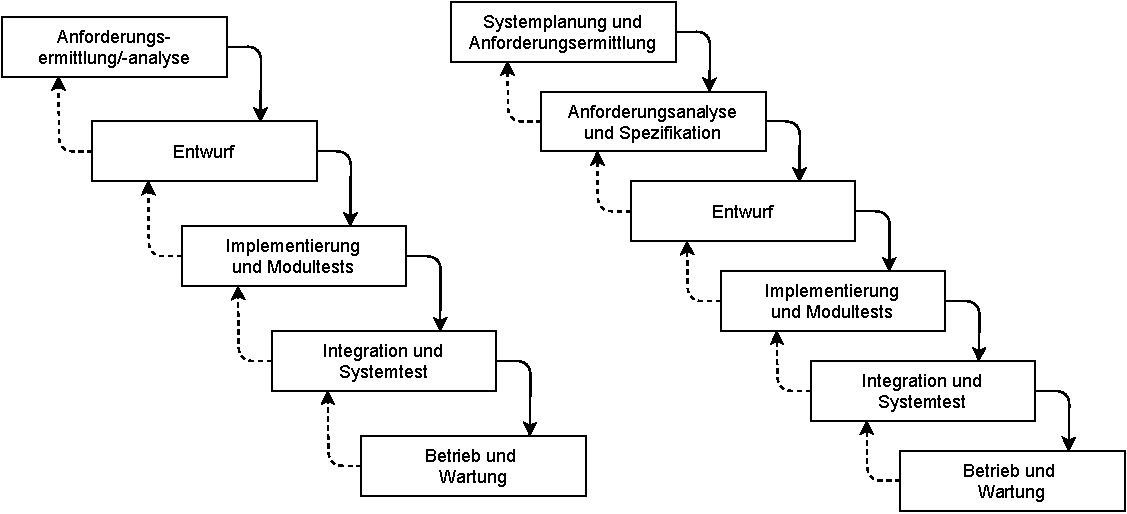
\includegraphics[width=1.0\textwidth]{Bilder/Kapitel-2/Abb-2-6.pdf}%
    \caption{Beispielhaftes fünf- bzw. sechsphasiges Wasserfallmodel}
    \label{fig:wasserfallmodel_fuenf_phasen}
\end{figure}

Im Vergleich zu fünfphasigen werden bei sechsphasigen Wasserfallmodellen meistens explizit Tätigkeiten der Planung des Softwareentwicklungsprojekts (\zb Kalkulation, Projektplan) integriert und der Prozess rund um die Spezifizierung von Anforderungen auf zwei Phasen aufgeteilt. Zum Beispiel sind die Erstellung von Lastenheft 
%\sttpkapitelverweis{Lastenheft und Pflichtenheft}{Kap.~\ref{sec:Kap-6.2.5}}
und Pflichtenheft bei fünfphasigen Modellen üblicherweise beide Teil der ersten Phase, während bei sechsphasigen Modellen die Erstellung des Pflichtenhefts erst zur zweiten Phase gehört. 

Die Wasserfallmodelle in Abbildung~\ref{fig:wasserfallmodel_fuenf_phasen} sind nur beispielhafte Ausprägungen fünf- und sechsphasiger Wasserfallmodelle. Die in konkreten Softwareentwicklungsprojekten eingesetzten Wasserfallmodelle unterscheiden sich von diesen Abbildungen, aber auch untereinander, oftmals im konkreten Zuschnitt und damit auch in der Benennung der einzelnen Phasen. Dies betrifft insbesondere den Bereich des Testens, bezogen auf die Abbildungen damit die Trennung zwischen der Phase Implementierung und Modultests %\sttpgls{Softwaretests} 
und der folgenden Phase Integration und Systemtest. Hier reicht das Spektrum von der kompletten Auslagerung des Testens in die spätere Phase – womit in der Implementierungsphase nur reine „Debugging-Tests“ stattfinden – bis zur Durchführung kompletter Integrationstests in der früheren Phase – womit in der späteren Phase nur noch der Systemtest verbleibt. 

\minisec{Struktur des Softwareentwicklungsprozesses}

\vspace{1.5mm} %%% für Druck

Das Wasserfallmodell ist ein sehr starres sequentielles Vorgehensmodell. Es sieht vor, dass mit einer Phase erst dann begonnen wird, wenn sämtliche Aktivitäten der vorherigen Phase abgeschlossen wurden und die entstandenen Ergebnisse qualitätsgesichert sind – dementsprechend alle Meilensteine erreicht sind. Der zu Beginn des Softwareentwicklungsprozesses einmal festgelegte Ablauf der abzuarbeitenden Aktivitäten wird nach Möglichkeit eingehalten.

\vspace{0.6mm} %%% für Druck

Aus Managementsicht besticht das Wasserfallmodell damit vordergründig durch seine Einfachheit. Anhand von Meilensteinen ist der Projektfortschritt jederzeit kontrollierbar. Zu Beginn eines Projekts kann eine systematische Planung der benötigten Personalressourcen erfolgen. Aufgrund des unterschiedlichen inhaltlichen Zuschnitts der einzelnen Phasen und der umfangreichen Dokumentation der Ergebnisse einer Phase ist es dabei möglich, für verschiedene Phasen unterschiedliche (auch örtlich unverbundene) Teams einzusetzen. Schon zu Beginn des Projekts kann zum Beispiel kalkuliert werden, wann ein erfahrener Softwarearchitekt und wann das Team der Softwaretester benötigt wird. Die abgegrenzten Zuschnitte der Phasen und die Ausrichtung auf zu erreichende Meilensteine führen zudem in der Regel dazu, dass in einem Projekt auch die einzelnen Arbeitsaufgaben innerhalb einer Phase stark vorgegeben sind. Gerade für Softwareentwickler mit wenig Erfahrung kann das Orientieren an festen Vorgaben und das Abarbeiten begrenzter Aufgaben hilfreich sein.

\vspace{0.6mm} %%% für Druck

Auch wenn das Wasserfallmodell die Rückkehr in schon abgeschlossene Phasen vorsieht, hängen Umfang und Anzahl der möglichen Überarbeitungen in der Praxis davon ab, wieviel zeitlicher Puffer für das Projekt eingeplant wurde. Der Einsatz eines Wasserfallmodells erfordert daher einen erfahrenen Projektleiter, der den Projektplan und die einzelnen Arbeitsschritte zielführend und realistisch durchführbar festlegt und dabei im Projektplan auch ausreichende Zyklen (Rückkehr in bereits abgeschlossene Phasen) für eventuell notwendige Überarbeitungen von Ergebnissen vorsieht. 

\vspace{0.6mm} %%% für Druck

In der Praxis ist die vorgesehene Abgeschlossenheit der Phasen zudem nicht immer notwendig, zum Beispiel weil Komponenten des zu entwickelnden Softwareprodukts so unabhängig voneinander sind, dass mit der Implementierung einer Komponente (\zb Benutzerverwaltung) begonnen werden könnte, bevor der Entwurf für eine andere Komponente (\zb Seminarverwaltung) komplett erstellt ist. Außerdem  treten in den meisten Projekten Verzögerungen im Projektablauf ein, sei es weil Mitarbeiter ausfallen, Aufwände für Tätigkeiten falsch eingeschätzt wurden oder Fehler bemerkt werden, die zeitaufwändig korrigiert werden müssen. Die geringe Flexibilität des Wasserfallmodells macht es schwierig auf solche Risikofaktoren zu reagieren. Sofern der Auslieferungstermin der Software nicht verschoben werden kann, führen Verzögerungen im Projektablauf oft zur Verkürzung der späteren Phasen des Projekts. Da im Wasserfallmodell der Bereich des Testens die letzte Phase vor der Auslieferung der Software bildet, gehen solche Verzögerungen in der Regel zu Lasten der Testaktivitäten.

\vspace{0.6mm} %%% für Druck

Hinzu kommt, dass durch die späte Testphase 
\marginline{späte Testphase}
Fehler sowie unvollständige oder unklare Spezifikationen erst spät im Projektverlauf offensichtlich werden. Spät erkannte Fehler sind oft teurer als frühzeitig erkannte Fehler, da größere Personalressourcen für Arbeiten auf fehlerhafter Grundlage investiert wurden. Sollten beim Testen oder auch erst im Betrieb noch größere Fehler in der Software entdeckt werden, ist es zudem zu spät Grundlegendes zu ändern. Es bleiben dann nur noch provisorische Behelfslösungen (engl. Workarounds), die die Symptome des fehlerhaften Verhaltens der Software behandeln, aber nicht die grundlegenden Probleme lösen. Um solche Situationen zu vermeiden, sehen viele heutige Wasserfallmodelle schon parallel zur Implementierung Testaktivitäten vor (\zb Tests einzelner Komponenten). Der abschließende sogenannte Systemtest, bei dem die Software gegen alle spezifizierten Anforderungen getestet wird, findet in Wasserfallmodellen in der Regel aber weiterhin erst in der letzten Phase vor der Auslieferung statt. Sollte dabei das Fehlen von Funktionalitäten bemerkt werden, ist es in den meisten Fällen zu spät, daran etwas zu ändern.

\minisec{Umgang mit Anforderungen}

Die Anforderungen an das zu erstellende Softwareprodukt werden im Wasserfall\-modell ganz zu Beginn des Softwareentwicklungsprojekts ermittelt. Sobald die Anforderungsspezifikation 
%\sttpkapitelverweis{Anforderungsspezifikation}{Kap.~\ref{sec:Kap-6.1.x}} 
erstellt und (vom Auftraggeber) geprüft wurde, können in der Regel keine neuen oder veränderten Anforderungen berücksichtigt werden. Das ist ein Problem: Zwischen der Planung eines Softwareentwicklungsprojekts und der Auslieferung des fertigen Produkts können durchaus mehrere Jahre liegen. In dieser Zeit können sich Arbeitsprozesse sowie Erfahrungen und Erwartungen von Nutzern schon derart verändert haben, dass das entwickelte Produkt die Bedürfnisse seiner Nutzer schon zum Zeitpunkt seines Ersteinsatzes nicht mehr erfüllt. Hinzu kommt, dass es nur selten wirklich möglich ist die Anforderungen zu Projektbeginn hundertprozentig vollständig und unmissverständlich zu erfassen.

\vspace{2mm}

\sttpDefinitionskasten{\sttpDefinitionskastenSkalierungsfaktor}{Kunde}{Auftraggeber oder Nutzer des Softwareprodukts.}{Wir verwenden den Begriff Kunde als Verallgemeinerung in Kontexten, in denen eine Unterscheidung zwischen Auftrag\-geber auf der einen Seite und Nutzer auf der anderen Seite nicht sinnvoll bzw. möglich ist.}

\minisec{Einbezug des Kunden}

Die Einbindung des Auftraggebers oder zukünftiger Nutzer des Softwareprodukts in den Prozess der Softwareentwicklung ist nur in der Zeit der Anforderungsermittlung/
\linebreak %%% für Druck
-analyse vorgesehen. In der Praxis kommt es natürlich trotzdem vor, dass auch in späteren Phasen bei Unklarheiten mit dem Auftraggeber Rücksprache gehalten wird, eine systematische Rücksprache in der Entwurfsphase (oder sogar in der Implementierungsphase) sieht das Wasserfallmodell aber nicht vor. Das kann auch bei im Projektverlauf stabilen Anforderungen leicht dazu führen, dass die wirklichen Vorstellungen der Kunden im fertigen Produkt unzureichend umgesetzt sind.

Wichtig für die erfolgreiche Softwareentwicklung mit einem Wasserfallmodell ist, dass im Softwareentwicklungsteam eine sehr genaue Kenntnis des fachlichen Problembereichs vorliegt, um die fehlende Einbindung und das somit nicht vorhandene Feedback des Kunden kompensieren zu können.

\vspace{2mm} %%% für Druck

\minisec{Artefakte des Entwicklungsprozesses}

Als sequentielles Vorgehensmodell ist das Wasserfallmodell dokumentenorientiert. Ein Großteil der Tätigkeiten während des Softwareentwicklungsprozesses ist darauf ausgerichtet, verschiedene Dokumente
\marginline{Dokumente}
zu erstellen (\zb Anforderungsspezifikation, Architekturspezifikation, Komponentenmodell, Testplan). Die Meilensteine am Ende der Phasen beziehen sich dementsprechend auch meistens auf das Vorliegen bestimmter Dokumente, welche dann in der Regel die Basis für die Aktivitäten der folgenden Phase bilden. Aufgrund dieser dokumentenorientierten Ausrichtung entsteht während der Entwicklung des Softwareprodukts eine umfangreiche technische Dokumentation des Systems. Dies erleichtert die Einarbeitung neuer Mitarbeiter während des Projekts, aber auch die Einarbeitung derjenigen Mitarbeiter, die das erstellte Softwaresystem später betreiben sollen.

\vspace{2mm} %%% für Druck

\minisec{Einsatz von Wasserfallmodellen}

Trotz aller Kritikpunkte am Wasserfallmodell sollte man seine Bedeutung nicht geringschätzen. Zum einen hat das Wasserfallmodell viel dazu beigetragen, unter Softwareentwicklern ein Verständnis für die notwendige Trennung zwischen den fachlichen Anforderungen auf der einen Seite und ihrer technischen Umsetzung auf der anderen Seite zu etablieren. Zum anderen haben sich auf Basis des Wasserfallmodells und insbesondere auch anhand seiner Probleme andere Arten von Vorgehensmodellen herausgebildet, die es ohne die – schon in den 1980er Jahren geführte – intensive Diskussion über die Vor- und Nachteile des Wasserfallmodells vielleicht nicht geben würde.

In  der Literatur finden sich unterschiedliche Ansichten darüber, in welchen Situationen und für welche Institutionen und Projekte es auch heute noch sinnvoll ist, ein Wasserfallmodell als Vorgehensmodell zu verwenden. Als typische
\marginline{Anwendungs\-bereiche}
Anwendungs\-bereiche werden oft eingebettete Systeme (engl. embedded systems) und sicherheitskritische Systeme genannt. Bei eingebetteten Systemen übernimmt die Software die Steuerung der Hardware sowie die Interaktion mit der Außenwelt. Da sich die Hardware nicht verändern lässt, sobald sie produziert wurde, müssen die Aufgaben\-teilung zwischen Hardware und Software und damit die genauen Anforderungen an die Software zu Beginn der Entwicklung festgelegt werden. Genauso orientiert sich der Entwurf der Software an den Gegebenheiten der Hardware. Da ein eingebettetes System aufgrund der Inflexibilität der Hardware damit in der Regel sowieso schwer auf veränderte Anforderungen reagieren kann, steht dieser Aspekt auch für die entsprechende Softwareentwicklung nicht so sehr im Vordergrund. Für die Entwicklung sicherheitskritischer Systeme gilt eine Reihe von Vorschriften, die bei der Softwareentwicklung eingehalten werden müssen. Dazu gehören oft auch formale Analysen von Spezifikations- und Entwurfsdokumenten, die nachweisen sollen, dass die notwendigen sicherheitskritischen Anforderungen berücksichtigt sind. Da es sich dabei um einen aufwändigen und teuren Prozess handelt, der idealerweise nur einmalig im Laufe der Entwicklung des Softwareprodukts stattfindet, sollten die Entwurfs\-tätig\-keiten vollständig abgeschlossen sein, bevor die formalen Analysen durchgeführt werden. Aber auch wenn in Projekten für eingebettete oder sicherheitskritische Systeme vielleicht häufiger Wasserfallmodelle zu finden sind, bedeutet das nicht, dass dort andere Vorgehensmodelle gar nicht eingesetzt würden. Auf der anderen Seite kann man auch in anderen Anwendungsgebieten auf wasserfallartige Vorgehensmodelle treffen.

In der Praxis wird die Entscheidung für ein Vorgehensmodell 
\marginline{Entscheidung für ein Vorgehens\-modell}
häufig nicht aufgrund der expliziten Abwägung seiner Vor- und Nachteile gegenüber den Vor- und Nachteilen anderer Vorgehensmodelle getroffen werden, sondern aufgrund weicherer Faktoren: Ein Unternehmen, das mit einem Wasserfallmodell erfolgreich ein Produkt für einen Kunden entwickelt hat, wird bei einem ähnlichen Produkt für einen anderen Kunden vermutlich wieder ein Wasserfallmodell wählen. Ein Projektleiter, der bei seinem letzten Projekt die Einbindung des Kunden schmerzlich vermisst hat, wird versuchen diesen Aspekt im neuen Projekt zu verbessern und damit evtl. auch zu einem anderen Vorgehensmodell wechseln. Wasserfallmodelle (oder andere Arten von sequentiellen Modellen) werden seit über vierzig Jahren in Soft\-ware\-entwick\-lungs\-projekten eingesetzt. Viele Unternehmen, die Software für interne oder externe Zwecke entwickeln, haben daher Arbeitsprozesse in anderen Abteilungen als der Softwareentwicklungsabteilung auf solche Vorgehensmodelle ausgerichtet (\zb die Bereiche Auftragsaquise, Vertragswesen, Personalplanung, Controlling). Gerade der Umstieg von einem sequentiellen Wasserfallmodell auf agile Vorgehensmodelle erfordert oft auch Veränderungen der Arbeitsprozesse des Unternehmens, die teuer und aufwändig sind und daher vielleicht nur zögerlich vorgenommen werden. Viele Softwarehersteller haben zudem im Laufe der Jahre wasserfallartige Modelle so an ihre Bedürfnisse angepasst, dass in ihren unternehmensspezifischen Modellen nicht mehr alle Nachteile des ursprünglichen Wasserfallmodells zum Tragen kommen.

Abgesehen von institutionellen oder anderen Zwängen lässt sich festhalten: Wenn mit einer etablierten Technologie für ein Umfeld mit stabilen Anforderungen entwickelt wird, diese Anforderungen zu Beginn des Projekts definiert werden können und ein erfahrener Projektleiter zur Verfügung steht, dann kann man über den Einsatz eines Was\-ser\-fall\-modells nachdenken. In allen anderen Fällen sollten flexiblere Vorgehensmodelle gewählt werden.
